
\section{Variants of Integral Transformations}
\begin{tabular}{|l||l|l|}
\hline & & \\
\textbf{Signal Type}
    & Discrete
    & Continuous \\
\hline \hline & & \\
Periodic
    & Discrete Fourier Transform
    & Fourier Series \\
\hline & & \\
Impulsive
    & ``Fourier Series with $T = \text{Pulse duration}$''
    & Fourier Integral \\
\hline & & \\
Causal
    & Z-Transformation
    & Laplace Transformation \\
\hline
\end{tabular}


\section{Discrete Fourier Transformation (DFT)}
    $$\boxed{s(h)=\sum_{k=0}^{N-1}\hat c_k e^{jhk\frac{2\pi}{N}}=\sum_{k=0}^{N-1}
    \left[ \hat{a}_k \cos\left(hk \frac{2 \pi}{N}\right)+\hat{b}_k \sin\left(hk
    \frac{2 \pi}{N}\right) \right]} \qquad N=\text{Number of periods}$$\\
    $$\hat{c}_k=\frac{1}{N}\sum_{h=0}^{N-1}s(h)
    e^{-jhk\frac{2\pi}{N}}=\hat{a}_k-j\hat{b}_k \qquad \hat{a}_k=\frac{1}{N}
    \sum_{h=0}^{N-1}s(h) \cos\left(hk \frac{2 \pi}{N}\right)=Re(\hat{c}_k) \qquad
    \hat{b}_k=\frac{1}{N} \sum_{h=0}^{N-1}s(h) \sin\left(hk \frac{2
    \pi}{N}\right)=-Im(\hat{c}_k)$$\\

    \subsection{Calculation with Matrices}
        \textbf{Transformation}\\
        1. Determine the period $N$ of the signal vector $\vec{s}=
        \begin{bmatrix}
        s(0) \\
        s(1) \\
        s(N-1)\\
        \end{bmatrix}$\\ \\
        2. Calculate the unit root $w$: $w=e^{j\frac{2 \pi}{N}}$\\ \\
        3. Calculate the matrix $W$: $W=
        \begin{bmatrix}
        w^0 & w^0 & w^0 & \ldots & w^0\\
        w^0 & w^1 & w^2 & \ldots & w^{N-1}\\
        w^0 & w^2 & w^4 & \ldots & w^{2(N-1)}\\
        \ldots & \ldots & \ldots & \ldots & \ldots\\
        w^0 & w^{N-1} & w^{2(N-1)} & \ldots & w^{(N-1)(N-1)}
        \end{bmatrix}$\\ \\
        4. Calculate matrix $V$: $V=W^*$ (conjugate complex)\\ \\
        5. Calculate the coefficients or Fourier transform $\vec{c}$:
        $\vec{c}=\frac{1}{N}V\vec{s}$\\

        \begin{minipage}{13cm}
            \textbf{Inverse Transformation}\\
            1. Calculate the matrix $W$ (as described in the transformation) \\
            2. Calculate the signal vector $\vec{s}$: $\vec{s}=W\vec{c}$
            \subsection{Matrix Multiplication}
            \begin{tabular}{ll}
                $\frac14
                \begin{bmatrix}
                    6 & -1 & 4 \\
                    3 & 2 & -2 \\
                    0 & -3 & -1
                \end{bmatrix}
                \cdot
                \begin{bmatrix}
                    1 \\
                    4 \\
                    3
                \end{bmatrix}
                =
                \frac14
                \begin{bmatrix}
                    6 \cdot 1 + (-1) \cdot 4 + 4 \cdot 3\\
                    3 \cdot 1 + 2 \cdot  4 + (-2) \cdot 3\\
                    0 \cdot 1 + (-3) \cdot 4 + (-1) \cdot 3
                \end{bmatrix}
                =
                \frac14
                \begin{bmatrix}
                    14\\
                    5\\
                    -15
                \end{bmatrix}
                =
                \begin{bmatrix}
                    3.5\\
                    1.25\\
                    -3.75
                \end{bmatrix}$
            \end{tabular}
        \end{minipage}
        \begin{minipage}[c]{5cm}
            \includegraphics[width=5cm]{../IntTra/bilder/matrix.png}
        \end{minipage}


	\subsection{Some W Matrices}
		\begin{tabular}{l l l l}
        N = 2 & N = 3 & N = 4 & N = 6\\
		$\begin{bmatrix}
		1 & 1\\
		1 & -1\\
		\end{bmatrix}$ &
		$\begin{bmatrix}
		1 & 1 & 1\\
		1 & -\frac{1}{2}+j\frac{\sqrt{3}}{2} & -\frac{1}{2}-j\frac{\sqrt{3}}{2}\\
		1 & -\frac{1}{2}-j\frac{\sqrt{3}}{2} & -\frac{1}{2}+j\frac{\sqrt{3}}{2}\\
		\end{bmatrix}$ &
		$\begin{bmatrix}
		1 & 1 & 1 & 1 \\
		1 & j & -1 & -j\\
		1 & -1 & 1 & -1\\
		1 & -j & -1 & j\\
		\end{bmatrix}$ &
		$\begin{bmatrix}
		1 & 1 & 1 & 1 & 1 & 1\\
		1 & \frac{1}{2}+j\frac{\sqrt{3}}{2} & -\frac{1}{2}+j\frac{\sqrt{3}}{2} & -1
		& -\frac{1}{2}-j\frac{\sqrt{3}}{2} & \frac{1}{2}-j\frac{\sqrt{3}}{2}\\
		1 & -\frac{1}{2}+j\frac{\sqrt{3}}{2} & -\frac{1}{2}-j\frac{\sqrt{3}}{2} & 1
		& -\frac{1}{2}+j\frac{\sqrt{3}}{2} & -\frac{1}{2}-j\frac{\sqrt{3}}{2}\\
		1 & -1 & 1 & -1 & 1 & -1\\
		1 & -\frac{1}{2}-j\frac{\sqrt{3}}{2} & -\frac{1}{2}+j\frac{\sqrt{3}}{2} & 1
		& -\frac{1}{2}-j\frac{\sqrt{3}}{2} & -\frac{1}{2}+j\frac{\sqrt{3}}{2}\\
		1 & \frac{1}{2}-j\frac{\sqrt{3}}{2} & -\frac{1}{2}-j\frac{\sqrt{3}}{2} & -1
		& -\frac{1}{2}+j\frac{\sqrt{3}}{2} & \frac{1}{2}+j\frac{\sqrt{3}}{2}\\
		\end{bmatrix}$
		\end{tabular}

		\begin{tabular}{l }
        N = 8\\
 		$\begin{bmatrix}
		1 & 1 & 1 & 1 & 1 & 1 & 1 & 1\\
		1 & \frac{\sqrt{2}}{2}+\frac{\sqrt{2}}{2}j & j &
		-\frac{\sqrt{2}}{2}+\frac{\sqrt{2}}{2}j & -1 &
		-\frac{\sqrt{2}}{2}-\frac{\sqrt{2}}{2}j & -j &
		\frac{\sqrt{2}}{2}-\frac{\sqrt{2}}{2}j\\
		1 & j & -1 & -j & 1 & j & -1 & -j\\
		1 &	-\frac{\sqrt{2}}{2}+\frac{\sqrt{2}}{2}j & -j &
		\frac{\sqrt{2}}{2}+\frac{\sqrt{2}}{2}j & -1 &
		\frac{\sqrt{2}}{2}-\frac{\sqrt{2}}{2}j & j &
		-\frac{\sqrt{2}}{2}-\frac{\sqrt{2}}{2}j\\
		1 & -1 & 1 & -1 & 1 & -1 & 1 & -1\\
		1 &	-\frac{\sqrt{2}}{2}-\frac{\sqrt{2}}{2}j & j &
		\frac{\sqrt{2}}{2}-\frac{\sqrt{2}}{2}j & -1 &
		\frac{\sqrt{2}}{2}+\frac{\sqrt{2}}{2}j & -j &
		-\frac{\sqrt{2}}{2}+\frac{\sqrt{2}}{2}j\\
		1 & -j & -1 & j & 1 & -j & -1 & j\\
		1 &	\frac{\sqrt{2}}{2}-\frac{\sqrt{2}}{2}j & -j &
		-\frac{\sqrt{2}}{2}-\frac{\sqrt{2}}{2}j & -1 &
		-\frac{\sqrt{2}}{2}+\frac{\sqrt{2}}{2}j & j &
		\frac{\sqrt{2}}{2}+\frac{\sqrt{2}}{2}j
		\end{bmatrix}$
		\end{tabular}



	\section{Fourier Series}
  	$$\boxed{f(t) = \sum\limits_{k = -\infty}^{\infty} c_k \cdot e^{j k \omega_1
  	t}}= \boxed{\sum\limits_{k = 0}^{\infty} \left(c_k \cdot e^{j k \omega_1
  	t} + \overline{c_k} \cdot e^{-j k \omega_1t}\right)}$$
  	$$\boxed{f(t) = \frac{a_0}{2} + \sum\limits_{k=1}^{\infty} \left[a_k \cos(k
  	\omega_1 t) + b_k \sin(k \omega_1 t)\right]}=\boxed{\frac{A_0}{2} +
  	\sum\limits_{k=1}^{\infty} A_k \cos(k \omega_1 t + \varphi_k)} \quad k\in
  	\mathbb{Z}, \quad \omega_1=\frac{2 \pi}{T}=2 \pi f$$

	$$\boxed{c_k=\overline{c_{-k}}=\frac{1}{T}\int_0^T{f(t)\cdot
	e^{-jk\omega_1
	t}dt}} \qquad \boxed{a_0 = \frac{2}{T}\int\limits_0^{T} f(t)dt, \quad a_k =
	\frac{2}{T}\int\limits_0^{T} f(t)\cos(k \omega_1 t) dt, \quad b_k =
	\frac{2}{T}\int\limits_0^{T} f(t)\sin(k \omega_1 t) dt}$$

	$a_0=c_0=A_0$ are \textit{constants}, $\omega_1$ is the
    \textit{fundamental angular frequency}, $a_k$ and $b_k$ are the \textit{real
    coefficients}, $c_k$ is the \textit{complex coefficient}, $A_k$ is the
    \textit{amplitude}, and $\varphi_k$ is the \textit{phase}.\\
	\fbox{
	\begin{tabular}{p{9cm}p{9cm}}
		$a_k = c_k + \bar{c_k} = 2\Real(c_k) = A_k \cos(\varphi_k)$ & $b_k = j(c_k + \bar{c_k}) = -2\Imag(c_k) = -A_k \sin(\varphi_k)$ \\ \\
		$c_k = \frac{a_k-jb_k}{2} = \frac{A_k}{2} e^{j\varphi_k} = \frac1T F(j k \omega)$ &
		$c_{-k} = \overline{c_k} = \frac{a_k+jb_k}{2} = \frac{A_k}{2} e^{-j\varphi_k}$ \\ \\
		$A_k = 2|c_k| = \sqrt{a_k^2+b_k^2}$ & $\varphi_k =  \arg(c_k)$\\
	\end{tabular}
	}

	\textbf{Calculation of $\varphi_k$ from $a_k$ and $b_k$}\\
    \begin{tabular}{p{4cm}p{4cm}p{3cm}p{3.5cm}}
        $a_k> 0:$ & $\varphi_k = -\arctan(\frac{b_k}{a_k})$ &
        $a_k<0:$ &    $\varphi_k = -\arctan(\frac{b_k}{a_k}) + \pi$\\
        $a_k = 0 \wedge b_k > 0:$ &    $\varphi_k = -\frac{\pi}{2}$ &
        $a_k = 0 \wedge b_k < 0:$ &    $\varphi_k = \frac{\pi}{2}$\\
        $a_k = 0 \wedge b_k = 0:$ &    $\varphi_k = \text{undefined}$
    \end{tabular}

	\subsection{Symmetry}
        \begin{tabular}{|p{4.3cm}|p{4.3cm}|p{4.4cm}|p{4.4cm}|}
            \hline
            \textbf{Even Function} & \textbf{Odd Function} &
            \textbf{Half Period 1} & \textbf{Half Period 2}\\
            \hline
            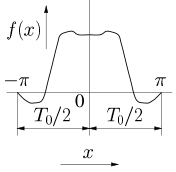
\includegraphics[width=3cm]{../IntTra/bilder/gerade_funktion.png}&
            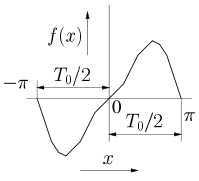
\includegraphics[width=3cm]{../IntTra/bilder/ungerade_funktion.png}&
            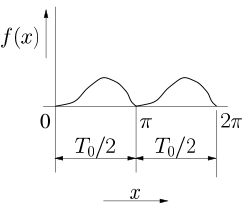
\includegraphics[width=3cm]{../IntTra/bilder/halbperiode_1.png}&
            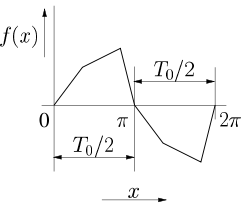
\includegraphics[width=3cm]{../IntTra/bilder/halbperiode_2.png}\\
            \hline & & & \\
            $f(-t)=f(t)$ & $f(-t)=-f(t)$ & $f(t)=f(t+\pi)$ & $f(t)=-f(t+\pi)$\\
            $b_k=0$ & $a_k=0$ & $a_{2k+1}=0$ & $a_{2k}=0$\\
            $a_k = \frac{4}{T} \int\limits_0^{\frac{T}{2}} f(t) \cdot \cos(k \omega_1
            t) dt$ &
            $b_k =  \frac{4}{T} \int\limits_0^{\frac{T}{2}} f(t) \cdot
            \sin(k \omega_1 t) dt$ &
            $b_{2k+1}=0$ & $b_{2k}=0$\\
            \hline
        \end{tabular}

    \subsection{Rectangular Signals}
    $$a_k=\frac{2}{T}\int\limits_{-t_1/2}^{t_1/2}A\cos\left(\frac{2\pi k}{T}t\right)dt=
    \left .\frac{2AT}{2\pi T k}\sin \left(\frac{2\pi k}{T}t\right)\right |_{-t_1/2}^{t_1/2}=
    \frac{2A}{\pi k}\sin\left(\frac{\pi t_1}{T}k\right)$$
    For ratios $\frac{T}{\text{gcd}(t_1,T)}=n\in\mathbb{N}$, the
    $n$th harmonic and its multiples disappear.\\
    \includegraphics[width=19cm]{../IntTra/bilder/fourierreihe-rechteck.png}
